Это задача с открытыми тестами. Это означает, что вам не требуется посылать решение, необходимо сдать только ответы на известный заранее набор тестов. Вы можете скачать тесты в секции материалов задачи. Это архив, содержащий файлы 01, 02, 03, \dots. Необходимо сдать один zip-архив содержащий ответы 01.out, 02.out, 03.out, \dots в корне архива. Архив может не содержать ответы на некоторые тесты, в этом случае вы получите вердикт ``\t{Неправильный ответ}'' на этих тестах.


Точками многоугольника являются как его внутренние точки, так и точки на границе.
Выпуклым многоугольником называется такой многоугольник, в котором для любых двух его точек $X$ и $Y$ отрезок,
соединяющий $X$ и $Y$, полностью принадлежит многоугольнику. Все многоугольники в этой задаче выпуклые и содержат
не менее 2-х вершин. Все вершины любого многоугольника в этой задаче различны и имеют целочисленные координаты.
Никакие три вершины не лежат на одной прямой. Слово <<многоугольник>> далее всегда обозначает именно такие многоугольники. 

Для двух данных многоугольников $A$ и $B$ их суммой Минковского называется фигура,
состоящая из всех точек вида $(x_1+x_2, y_1+y_2)$, где $(x_1, y_1)$ "--- все возможные точки многоугольника A, 
и $(x_2, y_2)$ "--- все возможные точки многоугольника B. 
Оказывается, что сумма Минковского двух многоугольников также является многоугольником.
Рисунок иллюстрирует сумму Минковского для двух треугольников.

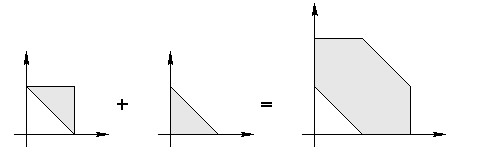
\includegraphics{task1a.jpg}

Будем рассматривать операцию, обратную сумме Минковского. 
Для данного многоугольника P требуется найти такие два многоугольника A и B, что:
\begin{itemize}
\item   P является суммой Минковского A и B;  
\item   A имеет от 2 до 4 различных вершин, то есть это отрезок (2 вершины), треугольник (3 вершины) или четырехугольник (4 вершины); 
\item   A должен иметь как можно больше вершин, то есть
       \begin{itemize}
       \item   A должен быть четырехугольником, если это возможно; 
       \item   если A не может быть четырехугольником, он должен быть треугольником, если это возможно;
       \item   иначе он должен быть отрезком. 
       \end{itemize}
\end{itemize}

Очевидно, что ни $A$ и ни $B$ не может быть равен $P$, поскольку в этом случае один из
многоугольников $A$ или $B$ должен быть точкой, что не является многоугольником по определению.

Вам дан набор входных файлов, каждый из которых содержит описание многоугольника $P$.
Для каждого входного файла вы должны найти многоугольники $A$ и $B$ такие, как описано выше,
и создать выходной файл, содержащий описания $A$ и $B$. Гарантируется, что для каждого из данных
входных файлов такие многоугольники существуют. Если существует несколько вариантов ответа,
запишите любой из них. Вы не должны сдавать какие-либо программы, вы должны сдать на проверку только выходные файлы. 